\newpage
\section{Ταξινόμηση}
\subsection{Εισαγωγή στους ταξινομητές}
Σε αυτή την ενότητα θα αναλύσουμε τους αλγορίθμους
ταξινόμησης και θα δούμε τη χρήση τους. Για τους αλγορίθμους
αυτούς χωρίζουμε το σύνολο των δεδομένων μας σε δυο μέρη:
\begin{itemize}
    \item Δεδομένα εκπαίδευσης (\textlatin{training dataset})
    \item Δεδομένα επαλήθευσής (\textlatin{testing dataset})
\end{itemize}
Τα πρώτα τα χρησιμοποιούμε έτσι ώστε ο αλγόριθμος να βρει
κάποιο μοτίβο στα δεδομένα με το οποίο θα μπορεί να
κατατάσσει τα καινούρια δεδομένα που δέχεται σε κάποια
από τις υπάρχουσες κλάσεις. Αυτή είναι και η διαδικασία
εκπαίδευσης του μοντέλου. Αφού η εκπαίδευση τελειώσει τότε
θα χρησιμοποιήσουμε τα δεδομένα επαλήθευσής για να
επιβεβαιώσουμε την ορθή λειτουργία του μοντέλου.
Υπάρχουν τρεις βασικοί τύποι ταξινομητών:
\begin{itemize}
    \item Δυαδικοί (\textlatin{binary})
    \item Πολλαπλών κλάσεων (\textlatin{multy-class})
    \item Πολλαπλών ετικετών (\textlatin{multy-label})
\end{itemize}

Οι δυαδικοί ταξινομητές χρησιμοποιούνται όταν έχουμε μόνο
δύο κλάσεις στις οποίες θέλουμε να εντάξουμε τα δεδομένα,
ή όταν η απάντηση που θέλουμε να πάρουμε από το μοντέλο
είναι δυαδικής φύσης. Για παράδειγμα, ένα πρόβλημα δυαδικής
φύσης θα ήταν να προβλέψουμε εάν ένας ασθενής έχει ή δεν
έχει μια ασθένειά σύμφωνα με τις εξετάσεις του.

Οι ταξινομητές πολλαπλών κλάσεων από την άλλη είναι ικανοί
να αναγνωρίσουν περισσότερες από δύο κλάσεις και είναι πολύ
χρήσιμοι για την αναγνώρισή προτύπων. Συνεχίζοντας με το
προηγούμενο παράδειγμα θα θέλαμε χωρίσουμε τους ασθενείς
σύμφωνα με την κατάσταση τους σε:
\begin{itemize}
    \item υγιείς
    \item ήπια ασθένειά
    \item σοβαρή ασθένεια
\end{itemize}
Έτσι οι γιατροί θα μπορούν αν δράσουν ανάλογα.

Οι ταξινομητές πολλαπλών ετικετών δεν έχουν κάποια καινούρια
λογική αλλά εφαρμόζουν τις λογικές των προηγούμενων
προβλημάτων. Δηλαδή θα μπορούσαμε να θέλουμε να υλοποιήσουμε
ένα μοντέλο το οποίο να κάνει και τις δύο προηγούμενες
προβλέψεις που συζητήσαμε. Αυτά τα μοντέλα συνήθως δε
χρησιμοποιούν ξεχωριστούς αλγορίθμους αλλά συνδυάζουν
πολλούς ήδη γνωστούς αλγορίθμους για να φτάσουν στο
αποτέλεσμα.
\begin{figure}[H]
    \centering
    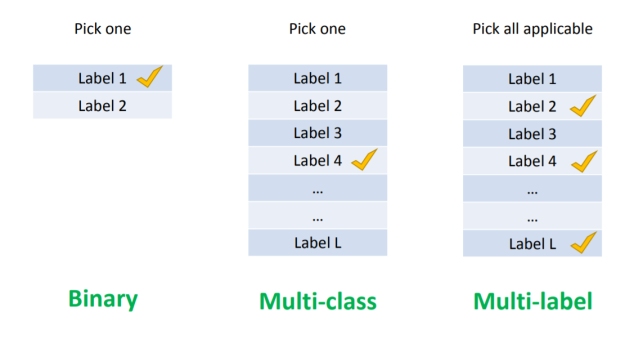
\includegraphics[width=0.5\textwidth]{images/typesOfClassifiers.png}
    \caption{Τύποι ταξινομητών}
\end{figure}

Στη συνέχεια θα αναλύσουμε τους διασημότερους αλγορίθμους
και τη χρήση τους. Οι αλγόριθμοι αυτοί είναι\cite{algo7, algo8, algo82}:
\begin{itemize}
    \item \textlatin{Naive Bayes}
    \item \textlatin{LDA (Linear Discriminant Analysis)}
    \item \textlatin{QDA (Quadratic Discriminant Analysis)}
    \item \textlatin{SVM (Support Vector Machine)}
    \item \textlatin{k-NN (k Nearest Neighbors)}
    \item \textlatin{Decision trees}
    \item \textlatin{Random Forest}
    \item Νευρωνικά δίκτυα (τα οποία θα αναλύσουμε στην παλινδρόμηση)
\end{itemize}

\subsection{\textlatin{Naive Bayes}}
Σύμφωνα με το παρακάτω άρθρο \cite{webb2010naive} ο αλγόριθμος \textlatin{Naive Bayes} είναι
ένας αλγόριθμος που κάνει την υπόθεση ότι τα χαρακτηριστικά είναι υπό όρους ανεξάρτητα της
δεδομένης κλάσης. Αυτή η υπόθεση στην πραγματικότητα δεν ισχύει αλλά ο αλγόριθμος πετυχαίνει
πολύ υψηλή ακρίβεια και ταυτόχρονα μεγάλη υπολογιστική απόδοση. Αυτός είναι και ο λόγος που
χρησιμοποιείται τόσο συχνά στην επιστήμη των δεδομένων.

Τα πλεονεκτήματα του αλγορίθμου είναι\cite{naive2023}:
\begin{itemize}
    \item Η χρονική πολυπλοκότητα αυξάνεται γραμμικά με το πλήθος των δειγμάτων και των
    στοιχείων τους
    \item Χαμηλό \textlatin{variance} (η αλλαγή των δεδομένων δεν επηρεάζει πολύ το μοντέλο)
    \item Μπορούμε εύκολα να προσθέσουμε και άλλα δεδομένα και το μοντέλο θα συνεχίσει την
    εκπαίδευση χωρίς πρόβλημα
    \item Δεν είναι επιρρεπής στον θόρυβο
    \item Δεν επηρεάζεται από έλλειψη τιμών στα δεδομένα
\end{itemize}

Τα μειονεκτήματά είναι:
\begin{itemize}
    \item Η υπόθεση ότι τα δεδομένα είναι ανεξάρτητα τον κάνει ακατάλληλο για ορισμένα
    προβλήματα
    \item Οι συνδυασμοί στοιχείων που δεν εμφανίζονται στο σύνολο δεδομένων για κάποια
    πρόβλεψη θα έχει πάντα μηδενική πιθανότητα.
    \item Οι πιθανότητες που υπολογίζει ενδέχεται να είναι λάθος
\end{itemize}

Ο αλγόριθμος χρησιμοποιεί τον κανόνα του \textlatin{Bayes}:
$$P(y|X)=\frac{P(y)\times{P(X|y)}}{P(X)}$$
Ο παραπάνω τύπος θα μας δώσει την πιθανότητα ενός δείγματος με στοιχεία $X$ να ανήκει στην
κλάση $y$. Το $X$ είναι διάνυσμα με όλα τα στοιχεία του δείγματος μας. Στο παρακάτω
παράδειγμα το $X$ για το πρώτο δείγμα θα είναι $\langle40,85\rangle$ και η κλάση θα είναι
$y=0$. Σκοπός μας είναι όταν πάρουμε τα στοιχεία από έναν ασθενή να μπορούμε να προβλέψουμε
αν έχει διαβήτη. Θα πρέπει δηλαδή να υπολογίσουμε τις πιθανότητες
$P\left(y=0|X=\langle x_1,x_2\rangle\right)$ και $P\left(y=1|X=\langle x_1,x_2\rangle\right)$
για τον καινούριο ασθενή με μετρήσεις $x1,x2$ και η πρόβλεψη θα είναι αυτή με τη μεγαλύτερη
πιθανότητα.

\begin{table}[H]
    \centering
    \begin{tabular}{|c|c|c|} \hline
        Γλυκόζη & Αρτηριακή πίεση & Διαβήτης \\ \hline
        40 & 85 & 0 \\ \hline
        40 & 92 & 0 \\ \hline
        45 & 63 & 1 \\ \hline
        45 & 80 & 0 \\ \hline
        40 & 73 & 1 \\ \hline
        45 & 82 & 0 \\ \hline
        40 & 85 & 0 \\ \hline
        30 & 63 & 1 \\ \hline
        65 & 65 & 1 \\ \hline
        45 & 82 & 0 \\ \hline
        35 & 73 & 1 \\ \hline
        45 & 90 & 0 \\ \hline
        50 & 68 & 1 \\ \hline
        40 & 93 & 0 \\ \hline
        35 & 80 & 1 \\ \hline
        50 & 70 & 1 \\ \hline
    \end{tabular}
    \caption{Δείγματα για πρόβλεψη διαβήτη}
\end{table}

Μέχρι εδώ ήταν η γνωστή στατιστική. Αλλά όσα περισσότερα στοιχεία έχουμε ανά δείγμα τόσο πιο
πολύπλοκος γίνεται ο υπολογισμός του παράγοντα $P(X|y)$. Εδώ δίνει λύση στο πρόβλημα ο
αλγόριθμος \textlatin{Naive Bayes} με την ανεξαρτησία των στοιχείων. Ανεξαρτησία σημαίνει
ότι
$$P(\langle x_1,x_2,\dots,x_n\rangle|y)=\prod\limits_{i=1}^nP(x_i|y)$$
Επίσης το $P(X)$ είναι πάντα σταθερό για τα δεδομένα στοιχεία που έχουμε άρα τελικά πρέπει
να υπολογίσουμε το
$$P(y)\times\prod\limits_{i=1}^nP(x_i|y)$$
για κάθε $y$ και στο τέλος να διαλέξουμε εκείνο το $y$ που έδωσε τη μεγαλύτερη τιμή
(που θα είναι και η κλάση στην οποία ανήκει το δείγμα). Βέβαια, αν τα στοιχεία δεν είναι
υπό όρους ανεξάρτητα δεν ισχύει αυτή η απλοποίηση. Παρ'όλα αυτά μπορεί να χρησιμοποιηθεί
σε πολλά σύνολα δεδομένων παρόλο που κάποιες φορές δεν ισχύει και για αυτόν τον λόγο
καλείται και αφελής \textlatin{Bayes}.

Ο αλγόριθμος είναι ιδανικός για προβλήματα πολλαπλών κλάσεων λόγω του εύκολου υπολογισμού.
Πιο συγκεκριμένα ο \textlatin{Naive Bayes} χρησιμοποιείται:
\begin{itemize}
    \item Στην ανίχνευση \textlatin{spam}. Μπορεί διαβάζοντας τις λέξεις ενός
    \textlatin{mail} να βρει την πιθανότητα να είναι \textlatin{spam}. Κάθε λέξη που διαβάζει
    θα αυξάνει ή θα μειώνει την πιθανότητα με κάποιον προκαθορισμένο κανόνα μέχρι που στο
    τέλος θα έχουμε πάρει μια ικανοποιητική απάντηση.
    \item Στη συναισθηματική ανάλυση. Οι εταιρίες μπορούν να κατατάξουν τα σχόλια των
    καταναλωτών τους σε θετικά και αρνητικά χρησιμοποιώντας τον αλγόριθμο. Μετά μπορούν
    να πράξουν ανάλογα έτσι ώστε να ευνοήσουν την εταιρία.
\end{itemize}

Υπάρχουν πολλές άλλες χρήσεις πέρα από αυτές. Για μια πιο αναλυτική εξήγηση των μαθηματικών
του αλγορίθμου μπορείτε να διαβάσετε την εξής έρευνα \cite{rish2001empirical}.

Οι αλγόριθμοι \textlatin{QDA} και \textlatin{QDA} χρησιμοποιούν επίσης τον τύπο του
\textlatin{Bayes}. Η διαφορά είναι στον τρόπο υπολογισμού του παράγοντα $P(X|y)$. Όπως και Ο
Αλγόριθμος \textlatin{Naive Bayes} κάνει μια υπόθεση για να τον υπολογίσει, το ίδιο κάνουν και
αυτοί οι αλγόριθμοι. Για να δείτε αυτούς τους τύπους με πλήρη εξήγηση μπορείτε να δείτε το
παράρτημα Α.

\subsection{\textlatin{Support Vector Machine}}
Οι μηχανές διανυσμάτων υποστήριξης (\textlatin{SVM}) είναι ένα σύνολο μεθόδων εποπτευόμενης
μάθησης
μέθοδοι που χρησιμοποιούνται για ταξινόμηση και παλινδρόμηση. Ανήκουν σε μια οικογένεια
γενικευμένων γραμμικών ταξινομητών. Ένα βασικό χαρακτηριστικό του είναι ότι είναι κάνει
προβλέψεις που χρησιμοποιούν τη θεωρία μηχανικής μάθησης για να μεγιστοποιήσει την
προγνωστική ακρίβεια ενώ ταυτόχρονα αποφεύγει την υπερβολική προσαρμογή στα δεδομένα
(\textlatin{over-fitting})\cite{jakkula2006tutorial}.

Τα πλεονεκτήματα του \textlatin{SVM} είναι\cite{svm1}:
\begin{itemize}
    \item Δουλεύει πολύ καλά όταν υπάρχει καθαρή διαφοροποίηση στα δεδομένα
    \item Δουλεύει καλύτερα σε μεγαλύτερες διστάσεις (πολλά στοιχεία ανά δείγμα)
    \item Είναι αποδοτικός όταν τα στοιχεία ανά δείγμα είναι περισσότερα από τα δείγματα
    \item Δεν κάνει μεγάλη χρήση μνήμης
\end{itemize}
Μειονεκτήματά:
\begin{itemize}
    \item Δεν είναι κατάλληλος για μεγάλο σύνολο δεδομένων
    \item Είναι επιρρεπής στον θόρυβο
    \item Λόγω του τρόπου υλοποίησης του δεν μπορούμε να πάρουμε την πιθανότητα αλλά μόνο
    την πρόβλεψη
\end{itemize}

Ο αλγόριθμος αυτός είναι αρκετά απλός και χρησιμοποιείται κυρίως για δυαδική ταξινόμηση. Αρχικά
για να τον καταλάβουμε θα πρέπει να αναπαραστήσουμε τα δεδομένα μας σαν σημεία σε έναν χώρο $N$
διαστάσεων, όπου $N$ τα στοιχεία που έχουμε ανά δείγμα. Το κάθε στοιχείο θα ανήκει σε μια από τις
δύο κατηγορίες τις οποίες θέλουμε να αναγνωρίσουμε. Ο αλγόριθμος λοιπόν προσπαθεί να φέρει ένα
υπερεπίπεδο τέτοιο ώστε να χωρίζει τα σημεία ανάλογα με την κατηγορία τους. Έτσι τα σημεία της
μιας κατηγορίας θα βρίσκονται από τη μια μεριά και της δεύτερης από την άλλη.

Για να κατανοήσουμε καλύτερα τον αλγόριθμο θα κάνουμε ένα παράδειγμα σε έναν χώρο δύο διαστάσεων
που μπορεί εύκολα να αντιληφθεί το ανθρώπινο μάτι.
\begin{figure}[H]
    \centering
    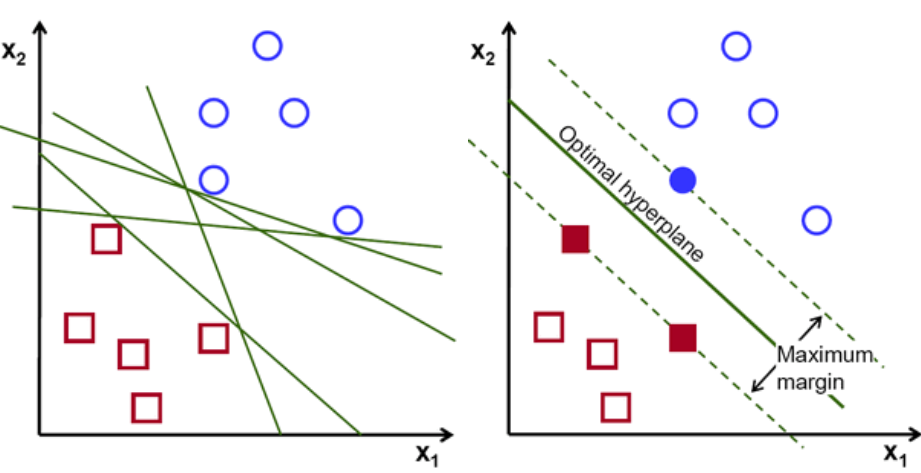
\includegraphics[width=0.75\textwidth]{images/svm.png}
    \caption{Παράδειγμα \textlatin{SVM}}
\end{figure}
Στον χώρο δύο διαστάσεων το υπερεπίπεδο είναι απλώς μια ευθεία. Εμείς λοιπόν θέλουμε να βρούμε μια
ευθεία που να χωρίζει τα τετράγωνα με τους κύκλους. Όπως μπορούμε να δούμε από το πρώτο διάγραμμα
υπάρχουν πολλές ευθείες που μπορεί να χωρίζουν τα σημεία μας αλλά εμείς θέλουμε να διαλέξουμε την
ευθεία που να έχει τη μέγιστη απόσταση και από τις δύο μεριές. Επομένως, όταν δώσουμε ένα
καινούριο δείγμα στον αλγόριθμο και θέλουμε να το κατατάξει σε μια από τις δύο ομάδες πρέπει απλά
να το τοποθετήσει σε αυτόν τον χώρο και μετά να δει από ποια μεριά της ευθείας βρίσκεται. Ανάλογα
με τη μεριά αυτή θα αποφασίσουμε και την κλάση του αντικειμένου.

Λύσαμε το πρόβλημα όπου είχαμε πάνω από μία ευθεία αλλά υπάρχει ένα μεγαλύτερο πρόβλημα. Αυτό
είναι η περίπτωση που δεν μπορούμε να χωρίσουμε τα στοιχεία μας με μια ευθεία. Εδώ έρχεται το
λεγόμενο "\textlatin{kernel trick}" για να λύσει το πρόβλημα. Το \textlatin{kernel} είναι μια
συνάρτηση σύμφωνα με την οποία επαυξάνουμε τη διάσταση του χώρου μας έτσι ώστε με την καινούρια
διάσταση που θα δημιουργηθεί τα σημεία μας να είναι διαχωρίσιμα από πλέον ένα επίπεδο. Όταν
γυρίσουμε πίσω στην αρχική διάσταση θα φαίνεται σαν τα σημεία μας να είναι διαχωρισμένα με μια
καμπύλη.
\begin{figure}[H]
    \centering
    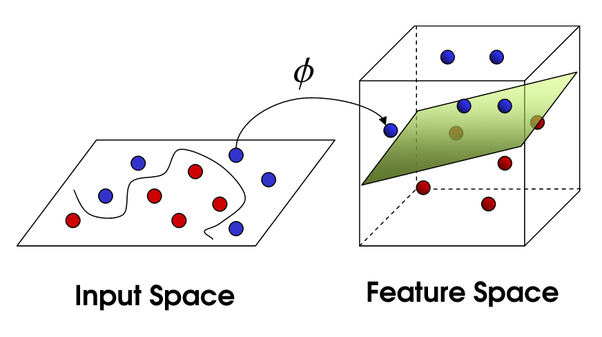
\includegraphics[width=0.75\textwidth]{images/svmdiminc.png}
    \caption{Επαύξηση διάστασης με \textlatin{SVM}}
\end{figure}

Ένα τελευταίο πρόβλημα που θα μπορούσαμε να λύσουμε θα ήταν να τροποποιήσουμε τον αλγόριθμο έτσι
ώστε να δουλεύει για πάνω από δύο κλάσεις. Ένας τρόπος να το κάνουμε αυτό θα ήταν με τη μέθοδο
\textlatin{ONE versus ALL}. Αυτό που κάνουμε είναι να φέρουμε μια ευθεία για κάθε κλάση που έχουμε
η οποία θα χωρίζει τον χώρο στα στοιχεία που ανήκουν σε αυτήν την κλάση και σε όλα τα υπόλοιπα.
Έτσι συνδυάζοντάς την πληροφορία και από τις τρεις ευθείες μπορούμε να πάρουμε τη σωστή απάντηση.
\begin{figure}[H]
    \centering
    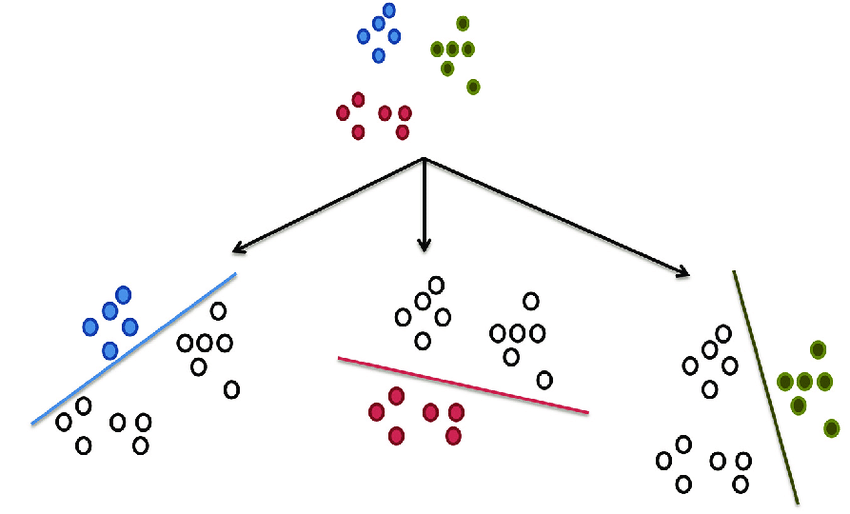
\includegraphics[width=0.7\textwidth]{images/svmonevsall.png}
    \caption{Ταξινόμηση πολλαπλών κλάσεων με \textlatin{SVM}}
\end{figure}
Βέβαια, κάνοντας αυτή τη μέθοδο θα εμφανιστουν σημεία στον χώρο τα οποία μπορεί να ανήκουν σε πάνω
από μια κλάση και και άλλα που δεν θα ανήκουν σε καμία. Θα πρέπει λοιπόν να λάβουμε υπόψη μας όχι
μόνο από ποια μεριά της κάθε ευθείας βρισκόμαστε αλλά και την απόσταση από αυτές για να μπορέσουμε
να καταλήξουμε σε ένα σωστό συμπέρασμα.

Μερικές χρήσεις του αλγορίθμου είναι\cite{svmuse}:
\begin{itemize}
    \item Ανίχνευση προσώπου
    \item Κατηγοριοποίηση κειμένου
    \item Ταξινόμηση εικόνων
    \item Βιοπληροφορική (πχ. ανίχνευση καρκίνου)
    \item Αναγνώριση γραφικού χαρακτήρα
    \item Γενικευμένος προγνωστικος έλεγχος (έλεγχος χαοτικών συστημάτων)
\end{itemize}

\subsection{\textlatin{K Nearest Neighbors}}
Ο αλγόριθμος \textlatin{k-NN} είναι ένας μη παραμετρικός αλγόριθμος ο οποίος χρησιμοποιεί την
εγγύτητα για να κατατάξει τα καινούρια στοιχεία σε μια από τις υπάρχουσες κλάσεις\cite{knnintro}. Αυτό
σημαίνει ότι το κάθε καινούριο στοιχείο θα παίρνει την κλάση του βλέποντας τις κλάσεις των πιο
κοντινών γειτόνων του διαλέγοντας την κλάση της πλειοψηφίας.

Τα πλεονεκτήματα του \textlatin{k-NN} είναι:
\begin{itemize}
    \item Εύκολη υλοποίηση
    \item Εύκολη προσαρμογή κατά την εμφάνιση καινούριων δεδομένων
    \item Δε χρειάζεται παραμέτρους παρά μόνο το \textlatin{k} και μια μετρική απόστασης
\end{itemize}

Κάποια μειονεκτήματά του είναι:
\begin{itemize}
    \item Δεν έχει καλή επεκτασιμότητα
    \item Δε δουλεύει καλά με μεγάλες διαστάσεις
    \item Μπορεί να γίνει εύκολα \textlatin{over fitting}
\end{itemize}

Για να ξεκινήσουμε τον αλγόριθμο πρέπει πρώτα να ορίσουμε ένα \textlatin{k}. Αυτό θα μας λέει
πόσα γειτονικά δείγματα να λάβουμε υπόψη μας για τον προσδιορισμό της κλάσης του καινούριου
δείγματος. Έπειτα βρίσκουμε τις αποστάσεις του σημείου από όλα τα σημεία με μια από τις μετρικές
που θα αναλύσουμε παρακάτω και διαλέγουμε τα \textlatin{k} σημεία με την κοντινότερη απόσταση στο
δικό μας. Τέλος, η κλάση του σημείου μας θα είναι η κλάση που έχει η πλειοψηφία των \textlatin{k}
σημείων.
\begin{figure}[H]
    \centering
    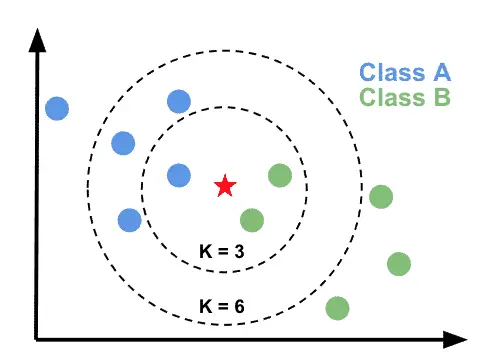
\includegraphics[width=0.5\textwidth]{images/knearest.png}
    \caption{Αλγορίθμος \textlatin{k-NN}}
\end{figure}

Για της μετρικές απόστασης γενικότερα στην επιστήμη των δεδομένων και στη μηχανική μάθηση έχουμε
τέσσερις βασικές επιλογές:
\begin{itemize}
    \item Ευκλείδεια απόσταση
    \item Απόσταση \textlatin{Manhattan}
    \item Απόσταση \textlatin{Minkowski}
    \item Απόσταση \textlatin{Hamming}
\end{itemize}

Η Ευκλείδεια απόσταση είναι η πιο γνωστή μετρική και γραφικά είναι το μήκος της ευθείας γραμμής
που ενώνει τα δύο σημεία μεταξύ τους. Δίνεται από τον γνωστό τύπο:
$$D=\sqrt{\sum\limits_{i=1}^{n}(x_i-y_i)^2}$$
Η απόσταση \textlatin{Manhattan} είναι επίσης πολύ γνωστή την οποί μπορούμε να
παραστήσουμε γραφικά όπως το παρακάτω σχήμα και έχει τύπο:
$$D=\sum\limits_{i=1}^{n}\left\lvert x_i-y_i\right\rvert$$
\begin{figure}[H]
    \centering
    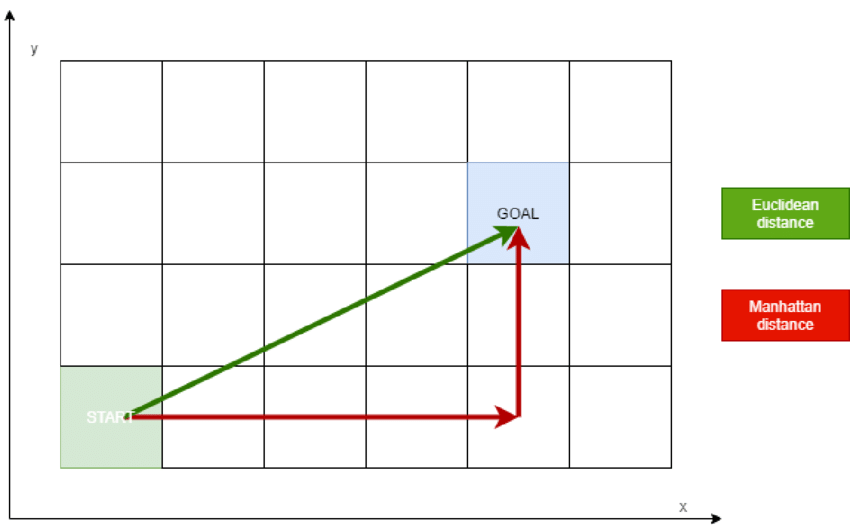
\includegraphics[width=0.5\textwidth]{images/manhattanDistance.png}
    \caption{Ευκλείδεια απόσταση και Απόσταση \textlatin{Manhattan}}
\end{figure}
Η απόσταση \textlatin{Minkowski} είναι ένα σύνολο αποστάσεων που αποτελεί μια γενίκευση των
παραπάνω δύο με τύπο:
$$D=\left(\sum\limits_{i=1}^{n}\left\lvert x_i-y_i\right\rvert^p\right)^{\frac{1}{p}}$$
Όπως μπορούμε αν δούμε πως για $p=1$ και $p=2$ παίρνουμε την απόσταση \textlatin{Manhattan} και
την ευκλείδεια απόσταση αντίστοιχα. Δεν μπορούμε να την αναπαραστήσουμε γραφικά αλλά για περαιτέρω
κατανόησή μπορούμε να δούμε το παρακάτω σχήμα όπου όλα τα σημεία στην μπλε γραμμή ισαπέχουν από το
κέντρο τους με μετρική την απόσταση \textlatin{Minkowski} για διαφορετικά $p$
\begin{figure}[H]
    \centering
    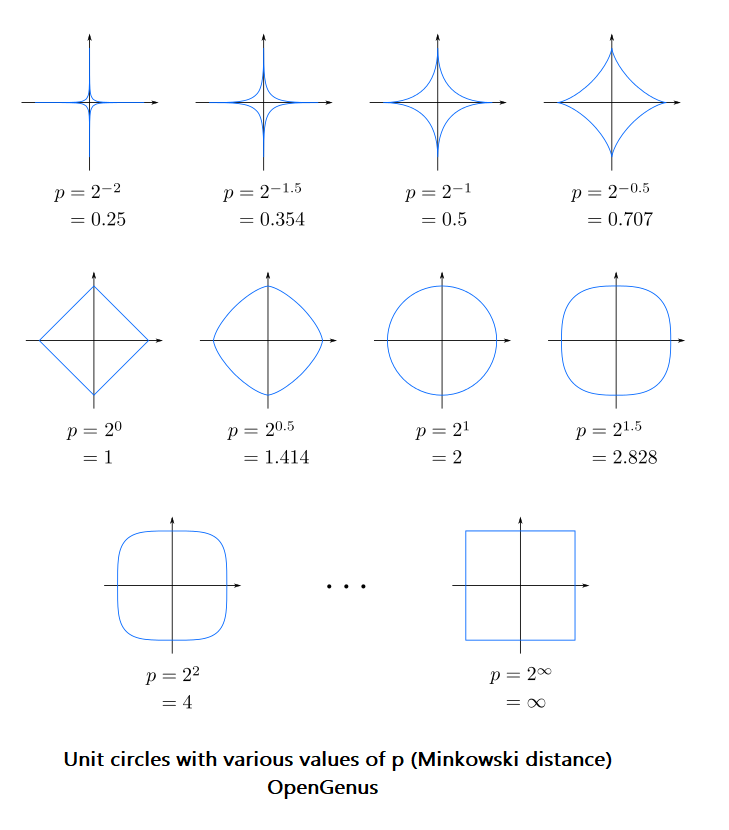
\includegraphics[width=0.6\textwidth]{images/minkowskiDistance.png}
    \caption{Απόσταση \textlatin{Minkowski}}
\end{figure}

Τέλος, η απόσταση \textlatin{Hamming} είναι πολύ απλή και εφαρμόζεται σε δυαδικά διανύσματα και
είναι το πλήθος των συνιστωσών που είναι διαφορετικές μεταξύ τους. Για παράδειγμα, αν έχουμε τα
διανύσματα $x=\langle 0,1,1,0,1\rangle,y=\langle 1,1,0,0,0\rangle$ η απόσταση τους θα είναι $3$
γιατί οι πρώτες, τρίτες και πέμπτες συνιστώσες είναι διαφορετικές μεταξύ τους.

Οι χρήσεις του \textlatin{k-NN} είναι πολύ παρόμοιες με αυτές του \textlatin{SVM}. Μια ακόμα χρήση
του είναι στην επιλογή προτεινόμενων που υπάρχουν σε πολλές μηχανές αναζήτησης. Μπορεί να βρει
τις προτάσεις που θα ταίριαζαν στον κάθε χρήστη ανάλογα με τα "κλικ" που κάνει βρίσκοντας έτσι τα
ενδιαφέροντα του.
\subsection{\textlatin{Decision Trees}}
Τα δέντρα αποφάσεων είναι μη παραμετρικοί αλγόριθμοι που χρησιμοποιούνται για ταξινόμησή και
παλινδρόμηση. Η αναπαράσταση τους γίνεται με τη μορφή δέντρου με κόμβους που χωρίζονται σε
κόμβους αποφάσεων και στους τελικούς κόμβους.

Κάθε δέντρο ξεκινάει από έναν κόμβο απόφασης με δύο ή περισσότερους δρόμους που οδηγούν σε άλλους.
Ο κάθε κόμβος απόφασης παρουσιάζει μια συνθήκη για τα δεδομένα και ο δρόμος που θα διαλέξουμε
εξαρτάτε από το αν η συνθήκη είναι αληθείς ή όχι. Αν συνεχίσουμε αυτή τη διαδικασία κάποια στιγμή
θα καταλήξουμε σε έναν τελικό κόμβο ο οποίος θα μας δίνει σαν απάντηση μία από τις κλάσεις που
έχουμε ορίσει για το σύνολο δεδομένων.
\begin{figure}[H]
    \centering
    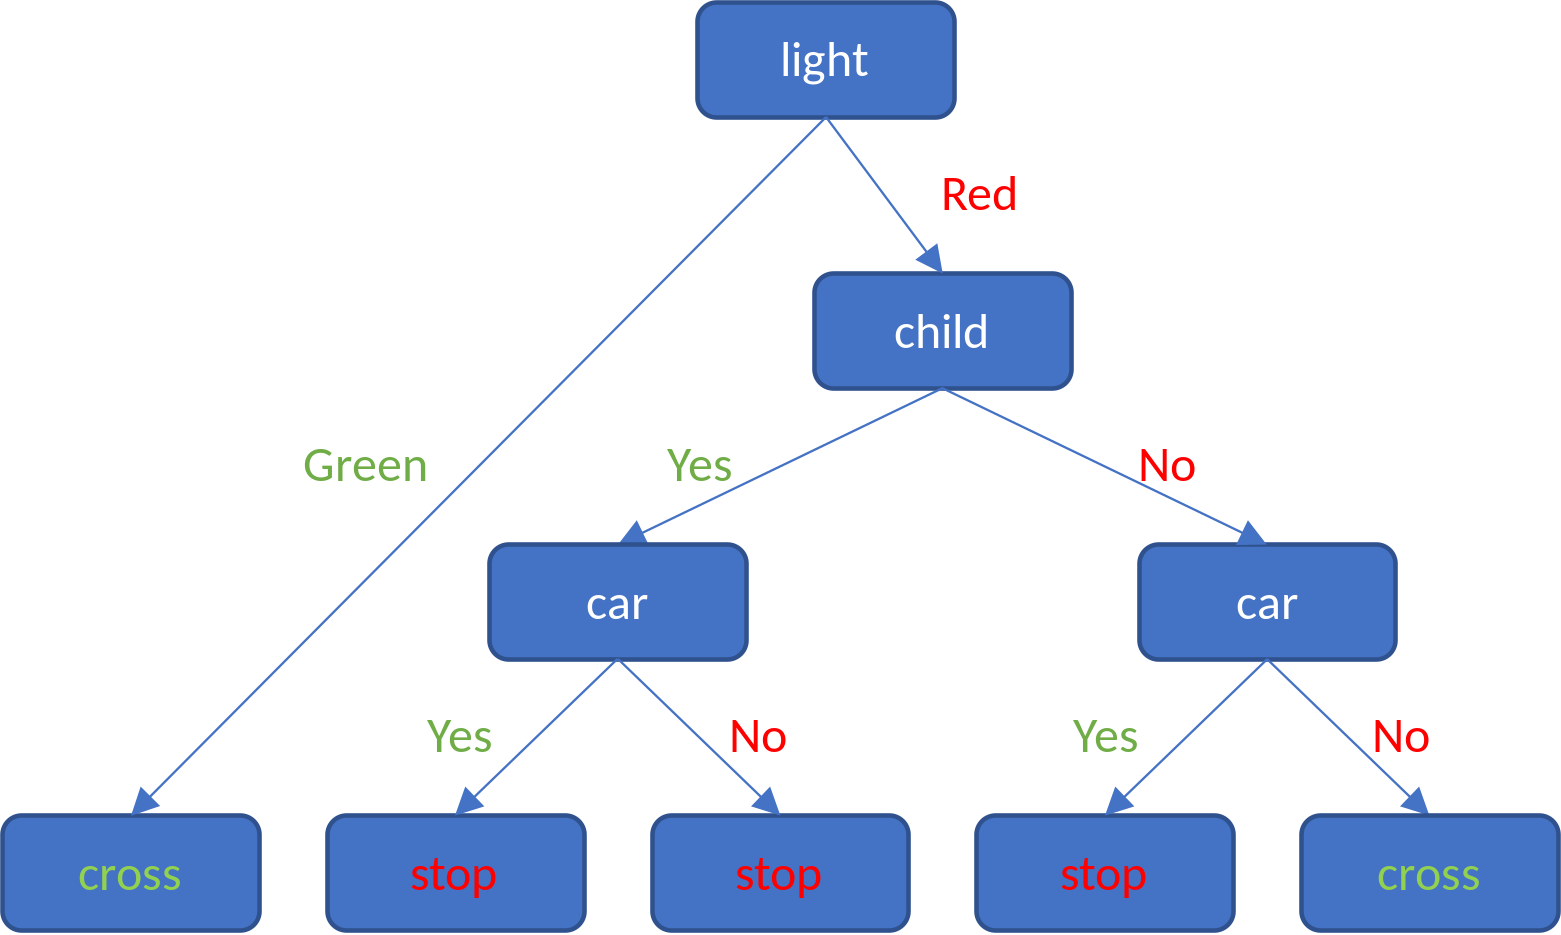
\includegraphics[width=0.6\textwidth]{images/decisionTree.png}
    \caption{Παράδειγμα δέντρου απόφασης}
\end{figure}
Για παράδειγμα στο σχήμα 10 θέλουμε ο υπολογιστής να πάρει την απόφαση για το αν ο άνθρωπος πρέπει
να περάσει τον δρόμο ή όχι. Για να το κάνει αυτό περνάει από πολλά στάδια αποφάσεων πριν καταλήξει
στην τελική του απόφαση.

Στην πραγματικότητα όμως τα δεδομένα δε θα είναι τόσο απλά. Τα δεδομένα μπορεί να μη διαχωρίζονται
με τις συνθήκες που έχουμε επιλέξει για τους κόμβους απόφασης. Αυτό όμως είναι ένα πρόβλημα γιατί
ένας τελικός κόμβος θα πρέπει να μας υποδεικνύει μόνο μία κλάση που σημαίνει ότι το σύνολο των
συνθηκών που περάσαμε για να φτάσουμε εκεί θα πρέπει να ισχύει μόνο για εκείνη την κλάση.

Για να μπορέσει ο υπολογιστής να βρει τις βέλτιστες συνθήκες για κάθε κόμβο πρέπει να
χρησιμοποιήσουμε τη θεωρεία της πληροφορίας. Θα κάνουμε ένα παράδειγμα για καλύτερη κατανόηση
του αλγορίθμου.

Έστω ότι έχουμε ένα πρόβλημα δυαδικής ταξινόμησης και έναν κόμβο απόφασης που στον οποίο έχουμε
20 στοιχεία και τα σημεία είναι διαχωρισμένα στις 2 κλάσεις στη μέση ($50\%-50\%$). Τώρα θέλουμε να
επιλέξουμε ανάμενα σε 2 συνθήκες:
\begin{itemize}
    \item Συνθήκη Α: Χωρίζει τα σημεία σε 2 κόμβους όπου:
    \begin{itemize}
        \item κόμβος 1: Έχει 14 σημεία με διαχωρισμό $42.8\%-57.2\%$
        \item κόμβος 2: Έχει 6 σημεία με διαχωρισμό $33.3\%-66.7\%$
    \end{itemize}
    \item Συνθήκη Β: Χωρίζει τα σημεία σε 2 κόμβους όπου:
    \begin{itemize}
        \item κόμβος 1: Έχει 4 σημεία με διαχωρισμό $0\%-100\%$
        \item κόμβος 2: Έχει 16 σημεία με διαχωρισμό $37.5\%-62.5\%$
    \end{itemize}
\end{itemize}
Μπορούμε να υπολογίσουμε την εντροπία από τον τύπο:
$$E=\sum\limits_{i=1}^{n}-p_i\log_2p_i$$
όπου $p_i$ η πιθανότητα της κλάσης $i$. Άρα έχουμε:
$$E_{parent}=-0.5\log_20.5-0.5\log_20.5=1$$
$$E_{A1}=-0.428\log_20.428-0.572\log_20.572=0.99$$
$$E_{A2}=-0.333\log_20.333-0.667\log_20.667=0.91$$
$$E_{B1}=-0\log_20-1\log_21=0$$
$$E_{B2}=-0.375\log_20.375-0.625\log_20.625=0.95$$
Παρατηρούμε ότι όσο καλύτερος είναι ο διαχωρισμός των στοιχείων, τόσο μικρότερη είναι η εντροπία.
Το κέρδος πληροφορίας για τις 2 συνθήκες είναι:
$$I_A=E_{parent}-\frac{14}{20}E_{A1}-\frac{6}{20}E_{A2}=0.034$$
$$I_B=E_{parent}-\frac{4}{20}E_{B1}-\frac{16}{20}E_{B2}=0.24$$
Ισχύει ότι $I_B>I_A$ και άρα θα προτιμήσουμε τη συνθήκη Β. Αυτός ο έλεγχος θα πρέπει να γίνει για
όλες τις πιθανές συνθήκες και για όλους τους κόμβους ξεκινώντας από τον αρχικό κόμβο. Είναι
σημαντικό να αναφέρουμε ότι αυτός είναι ένας άπληστος αλγόριθμος διότι επιλέγει την καλύτερη
συνθήκη για έναν κόμβο αλλά μπορεί μια χειρότερη επιλογή να οδηγούσε σε καλύτερο αποτέλεσμα αν
βλέπαμε τη συνολική εικόνα.

Ένα πρόβλημα με τα δέντρα είναι ότι έχουν μεγάλο \textlatin{variance} και γι' αυτό τον λόγο πολλές
φορές δεν μπορούν να γενικευτούν για καινούρια δεδομένα. Έτσι σαν μια εξέλιξη του αλγορίθμου
δημιουργήθηκε ο αλγόριθμος του τυχαίου δάσους (\textlatin{Random Forest}). Ο αλγόριθμος αυτός
είναι συνδυασμός μεθόδων και όπως φαίνεται από το όνομα του αποτελείται από πολλά
\textlatin{decision trees}. Μετά για την τελική απόφαση αν έχουμε πρόβλημα ταξινόμησης θα
επιλέξουμε την κλάση που δείχνει η πλειοψηφία, ενώ αν έχουμε πρόβλημα παλινδρόμησης θα πάρουμε
τον μέση τιμή των απαντήσεων\cite{wikirf}.

Το παραπάνω εξηγεί τη λέξη δάσος όμως δεν εξηγεί τη λέξη τυχαίο. Ο λόγος που είναι τυχαίο είναι
επειδή το κάθε δέντρο δε συμπεριλαμβάνει όλα τα δείγματα αλλά ένα τυχαίο τμήμα αυτών και επιπλέον
για αυτά τα δείγματα δε θα έχουν όλα τα χαρακτηριστικά τους αλλά θα επιλεχθούν κάποια τυχαία.
Παρακάτω βλέπουμε ένα παράδειγμα για το πώς θα χωρίζαμε τα δεδομένα μας για ένα τυχαίο δάσος που
θα αποτελείται από τέσσερα δέντρα.
\begin{table}[H]
    \centering
    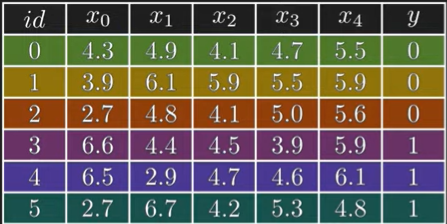
\includegraphics[width=0.5\textwidth]{images/random_forest.png}
    \caption{Σύνολο δεδομένων για τον αλγόριθμο \textlatin{random forest}}
\end{table}
\begin{table}[H]
    \centering
    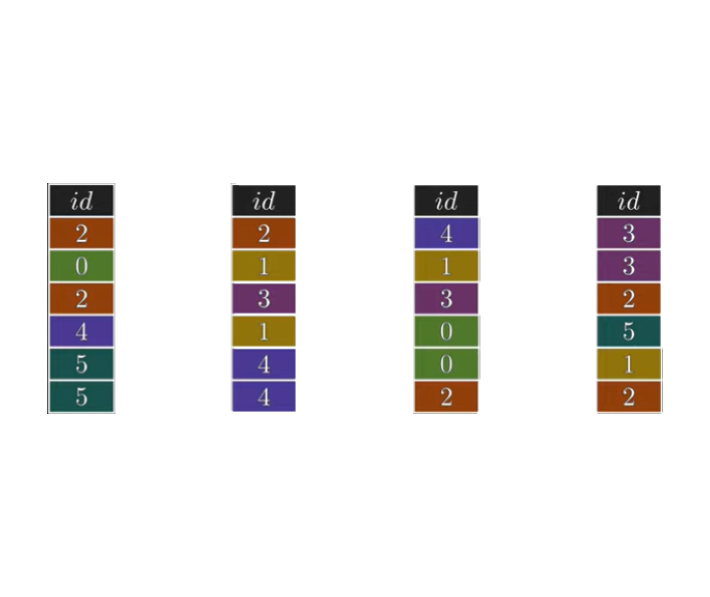
\includegraphics[width=0.5\textwidth]{images/random_forest_split.png}
    \caption{Σύνολο δεδομένων για κάθε δέντρο}
\end{table}

Επίσης, όπως είπαμε το κάθε υποσύνολο δεδομένων δε θα περιέχει όλα τα στοιχεία. Για παράδειγμα, το
πρώτο θα μπορούσε να έχει μόνο τα στοιχεία $x_1,x_2$, το δεύτερο τα $x_1,x_4$ κ.ο.κ.

Τα πλεονεκτήματα των δέντρων είναι ότι δε χρειάζεται προ επεξεργασία των δεδομένων. Στα δεδομένα
πολλές φορές λείπουν στοιχεία που πρέπει ή μπορεί να χρειάζεται κάποια κανονικοποίηση για να
εφαρμόσουμε κάποιους αλγόριθμους. Τα δέντρα όμως δεν είναι ένας από αυτούς και αυτό τα κάνει πολύ
καλή επιλογή σε τέτοιες περιπτώσεις. Επιπλέον, όπως είπαμε είναι μη παραμετρικοί και επίσης
δεν είναι γραμμικοί που είναι κάτι που θέλουμε πολλές φορές για καλύτερο διαχωρισμό των
κλάσεων\cite{dtreeadv}.
Το βασικό πρόβλημα του αλγορίθμου είναι το \textlatin{overfitting} το οποίο λύνει ο αλγόριθμος
\textlatin{random forest}.
